\chapter*{Introduction \& problem definition}
This is the report of Paolo Ginefra's solution to the "Image Analysis and Computer Vision" homework 2024/25.
All the referenced code is available in the GitHub Repository.

\section{Problem definition}
In this section, the problem at hand will be described in detail referencing the "Homework Assignment 2024-25" document.
\subsection{Scene description}
 A piece of furniture is a rectangular parallelepiped, whose width (along the X-axis) is $l = 1$. 
The other dimensions, namely the depth $m$ along the $Y$ axis and the height $h$ along the $Z$-axis are 
unknown. In addition, a horizontal circumference $C$(i.e., parallel to the X-Y plane) is visible. 
Furthermore, an unknown horizontal planar curve $S$ is also visible, placed at midheight $h$/2. 

\begin{figure}[!ht]
\centering
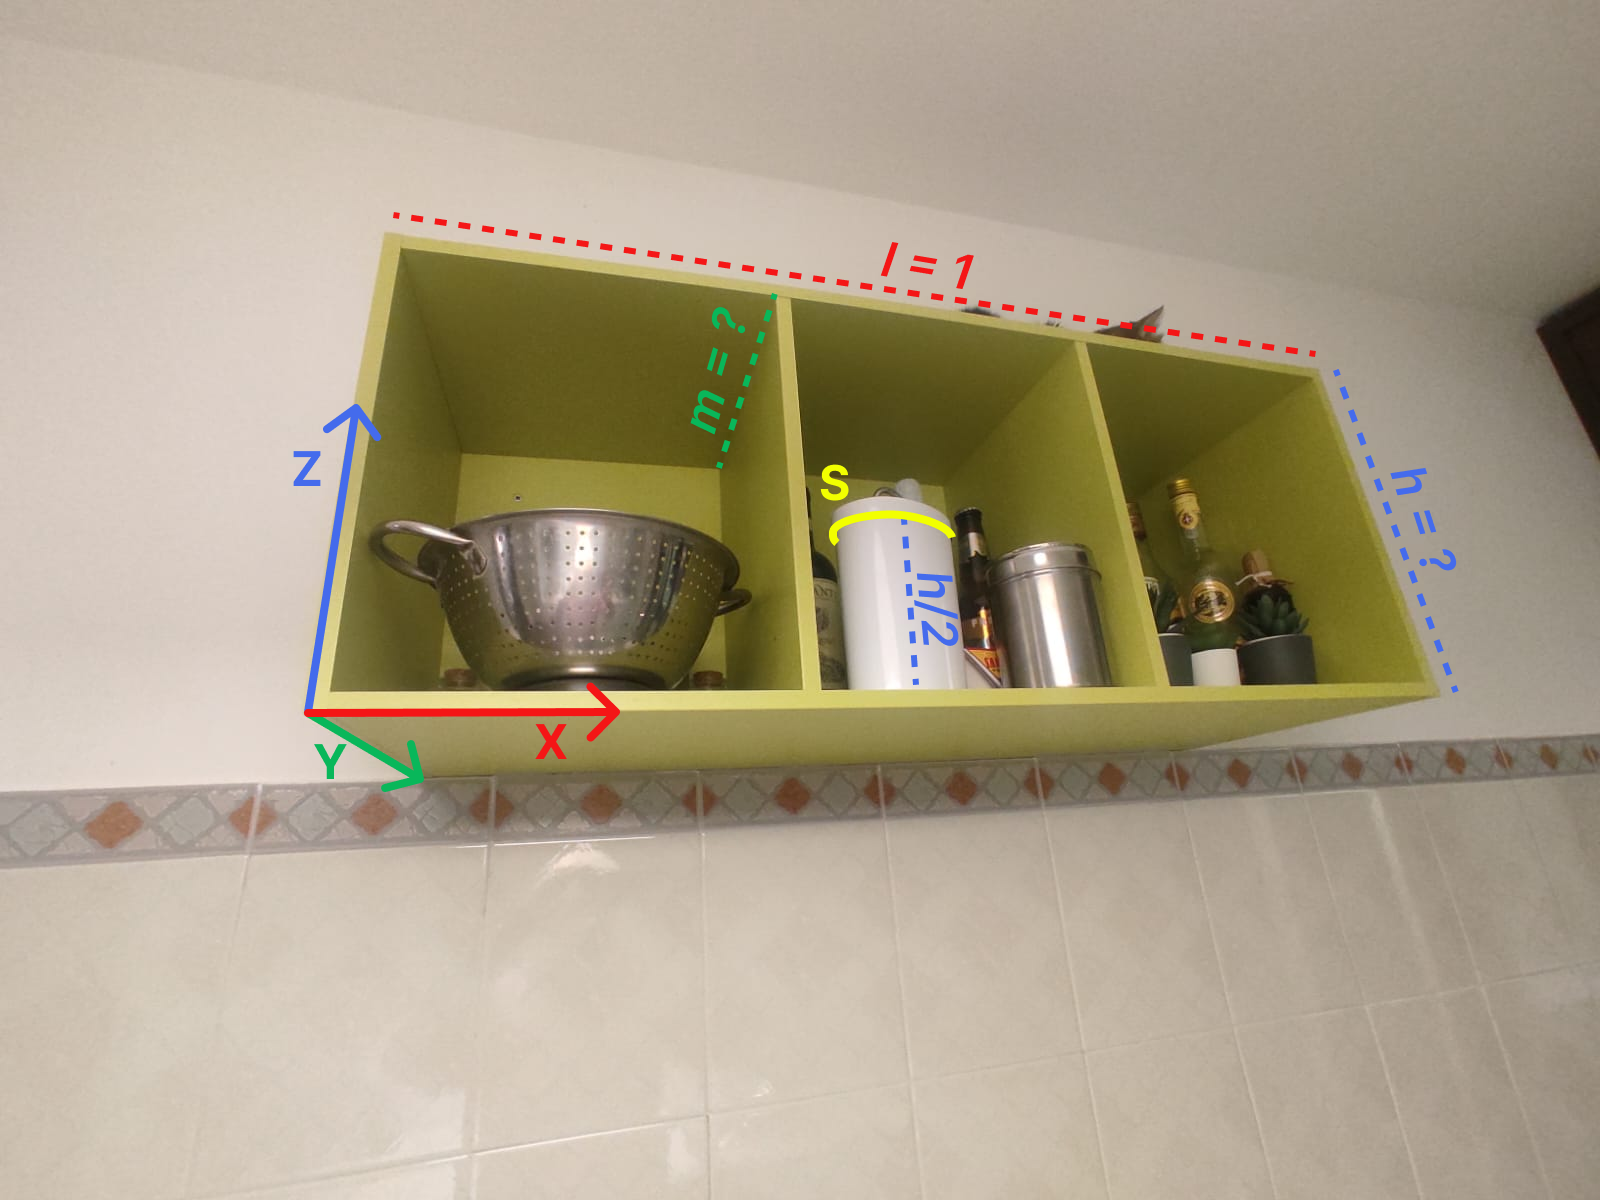
\includegraphics[height=9.5cm, width=\textwidth, keepaspectratio]{Report/Images/Introduction/SceneDescription.png}
\caption{\label{fig:SceneDescription}The Scene Description}
\end{figure}
